\section{Wisdom, Prudence, Cunning}

\begin{quotex}
Fools despise wisdom and instruction. \flright{\textsc{Proverbs 1:7}}

Blessed is the man that findeth wisdom, and is rich in prudence. \flright{\textsc{Proverbs 3:13}}

I am sending you out like sheep among wolves. So be as cunning as serpents and as innocent as doves. \flright{\textsc{Matthew 10:16}}

And it thus appears that the entire world is like a single mirror full of lights presenting the divine wisdom, or as
charcoal emitting light. \flright{\textsc{Bonaventura}, \emph{Collationes in Hexaemeron} ii, 27}

\end{quotex}

The German chemist Wilhelm Ostwald\footnote{\url{https://en.wikipedia.org/wiki/Ostwald_color_system}} last century developed a colour model. Although it was
developed specifically for manufacturing, and there have since been other models, the concept itself is sound.

This diagram shows Ostwald's colour picker as a bicone. The polar points are white, which is all
colours, and black, which is the absence of colour. The central axis, therefore represents shades of grey. Along the
circumference of the circle at the centre of the bicone, that is, the equator, are all the colours in the spectrum.
Physics considers only these to be true colours, since each corresponds to a specific wavelength. The spectrum is
created by passing white light through a prism. Unfortunately for the physicist, there is no formula to detect colours,
which requires a human observer to name them. Nevertheless, all the other representations are better called ``hues"
rather than colour.

This figure is similar to the quaternio so favoured by Carl Jung. He uses an octahedron, so there is a square where the
circle is. The square, as fourfold, represents completeness. The circle is also complete, but it also implies
perfection. The bicone is used whenever continuity is required.

The diagram shows white light, which is a composite of all the colours, at the top, and black, the total absence of
colour at the bottom. As the white light is separated into its components, it manifests as pastels, then the full
colour spectrum, and the, with decreasing intensity moves down to the browns and darker hues.

\paragraph{Polarity}
The poles of the bicone represent opposing forces, the active and the passive. The task of Hermetic philosophy is to
locate the neutralizing force or equilibrium that reconciles the opposites. For our example, the North Pole represents
Wisdom, and the South Pole, cunning.

\paragraph{Wisdom}
Wisdom is the first and the greatest of the gifts the Holy Spirit. It illumines the mind and leads the will to the
divine. Like the white light of the North Pole, Wisdom, the Mind of God, contains all possibilities.

The word of the Holy Trinity became flesh in Jesus Christ and its light became flesh in Mary.

\paragraph{Cunning}
\begin{quotex}
mimicry is precisely what the Book of Genesis understands by cunning when it says that ``the serpent was more cunning
than any other wild creature that the LORD God had made". To be cunning is to mime wisdom, after having eliminated the
essential — its light — and then to make use of it for
one's own ends. Cunning is the ape of Wisdom. \flright{\textsc{Valentin Tomberg}}

\end{quotex}
Human beings who are dominated by the Thinking function of the soul, become detached from conscience and will. That
opens them up to Luciferic influences, which is the seducing principle. Without the light of Sophia, they can indeed be
called ``children of the serpent" or ``children of darkness". The will is not oriented toward God but rather to earthly
power and riches. Feelings are irrelevant to cunning; the only goal is success, even if achieved through deceit or
guile.

Cunning holds such a strong attraction because it is so effective. Those able to manipulate the world and other people
can find worldly success. Since he is thinking and focused, while most everyone else is dominated by feelings and lower
desires, he holds an advantage. Those dominated by the Feeling function, become hypnotized and are prey to propaganda
and deceit. Those dominated by lower desires develop a separate I of the body that makes it impossible to become a real
person.

As long as human beings are not fully conscious, they will listen to the serpent. His promise of special or secret
knowledge mimics wisdom, so even those with good intentions can still fall into the temptation of cunning. Jung
explains this process in psychological terms:

\begin{quotex}
Since the shadow, in itself, is unconscious for most people, the snake would correspond to what is totally unconscious
and incapable of becoming conscious, but which, as the collective unconscious and as instinct, seems to possess a
peculiar wisdom of its own and a knowledge that is often felt to be supernatural. This is the treasure which the snake
guards, and also the reason why the snake signifies evil and darkness on the one hand and wisdom on the other. Its
unrelatedness, coldness, and dangerousness express the instinctuality that with ruthless cruelty rides roughshod over
all moral and any other human wishes and considerations and is therefore just as terrifying and fascination in its
effects as the sudden glance of a poisonous snake. \flright{\textsc{Carl Jung}, \emph{Aion}}

\end{quotex}
\paragraph{Prudence}
\begin{quotex}
Behold, I send you out as sheep in the midst of wolves; so be wise as serpents and innocent as doves. \flright{\textsc{Matthew 10:16}}

\end{quotex}
Prudence is the reconciling principle between Wisdom and cunning. The World is represented as the plane at the centre of
the bicone. The battle is not between the Light and the darkness, but takes place in the world. One must use
intelligence to be able to wander about in the midst of wolves. It is insufficient to be naively innocent, counting on
God alone to resolve all your problems. As Tomberg makes clear:

\begin{quotex}
The first three petitions [of the Our Father prayer] affirm divine authority, not divine power. Hence, God is powerful
to the extent that his power is freely recognized and accepted. \flright{\textit{Letter IV}}

\end{quotex}
While we recognize His authority in the world, His Will is without effect unless that power is allowed to act through
us. But first, it is necessary to bring the unconscious into consciousness; specifically, that entails bringing the Our
Father prayer all the way down to our lower centres. Then the innocence of the Dove can penetrate all the way down to
our lower centres. In that case, we can use the cunning of the serpent in innocence.

As was just mentioned, unbalanced humans are subject to seduction, hypnosis, and false egos. This is overcome only by
balancing the three soul functions. Training in the path of the Heart aims for the thinking, feeling, and willing
functions to be animated by the Higher Self. Then there can be gradual improvement:

\begin{wrapfigure}{rt}{.3\textwidth}
 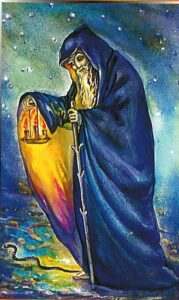
\includegraphics[scale=.7]{a20201012WisdomPrudenceCunning-img001.jpg}
\end{wrapfigure}

\begin{itemize}
\item Thinking and Feeling: \textbf{Positivity} 
\item Thinking and Willing: \textbf{Impartiality} 
\item Thinking, Willing, and Feeling: \textbf{Harmony} 
\end{itemize}
Prudence begins with a positive attitude, impartial judgment, and a harmonious inner life. Prudence is one of the
cardinal virtues, and can be thought of as ``applied wisdom", i.e., wisdom applied to concrete situations. A wanderer in
the world, a knight errant, must be prudent. The world is not just sheep and wolves, but is shared by many other
people. One must certainly know one's enemies, but not everyone, who is not a friend, is an enemy.

Unfortunately, prudence has become the lost virtue. Any mention of prudence as a virtue often brings on an attack. One
is suspected of ``blaming the victim", or of preventing someone's right to act in a certain way. A
few weeks ago, I saw a woman interviewed on TV. She was a student at a prestigious college who got so inebriated that
she passed out on the street. A passerby then raped her, and she didn't even know about it.

Clearly, it was not prudent of her to put herself in that condition in the first place. Of course, the crime of rape had
been committed. She was incensed to accept any responsibility. We agree; she did not commit the crime, nor did she
contribute to or it. It is not a question of ``blaming the victim", but rather the prudential judgment of not being a
victim in the first place. Many more examples can be found in everyday life.

\paragraph{The Hermit}

The Arcana of the Hermit represents Prudence. The Hermit abides in the Light, wanders in the world like the knight
errant, and makes forays into the lower realms. Tomberg explains the symbolism:

\begin{quotex}
The Hermit holds the \textbf{lamp} which represents the ``luminous point" of transcendental synthesis; he is wrapped in a
\textbf{mantle}, hanging in folds, for deploying the particular qualities which have their place in the region of the
``equator"; and he supports himself with a \textbf{staff} for feeling his way in the domain of darkness, in the region
of the reversed cone culminating in the ``black point".

He is therefore a Peripatetic Platonist (en route around the ``equator"), making use of scepticism (his
``staff') while he walks. This is why the traditional interpretation of the ninth Arcanum is
\emph{prudence}.

\end{quotex}


\flrightit{Posted on 2020-10-12 by Cologero }

\begin{center}* * *\end{center}

\begin{footnotesize}\begin{sffamily}



\texttt{Tom on 2020-10-12 at 15:20 said: }

I appreciated this post as it helped confirm and deepen some of the conclusions and meditations I recently made on the
Inferno of the Divine Comedy. 

At various points in the Inferno, Dante, relying on Virgil, is able to enlist the help of numerous demons, such as the
Centaurs and Titans. Enlisting their help is a terrifying experience for Dante, but with Virgil's
ability to command (or at least negotiate with) them, the threat they pose is neutralized, and they are instead shown
to be indispensable auxiliaries in the journey through the underworld.

The interpretation I made, based on some of my own experiences, is that Dante is describing how in our earthly life, we
often need to make use of these ``lower" powers while remaining firmly in command of them. An example that comes to mind
is in physical battle – a man would find it difficult to fight without awakening the fierce Centaur nature, the key
being then to remain firmly in command of it. Someone who has engaged in any kind of battle has probably experienced
this Centaur nature first hand. Similar interpretations can probably be made for the Titans, Geryon, and other helpful
demons in Dante's underworld.


\end{sffamily}\end{footnotesize}
